\documentclass[12pt]{article}
\usepackage[margin=1.5in]{geometry}

\usepackage[shortlabels]{enumitem}
\setcounter{secnumdepth}{0}

\usepackage{graphicx}
\usepackage{caption}

\usepackage{fancyhdr, lastpage}
\pagestyle{fancy}
\fancyhf{}
%
\lhead{Group Meeting}
%\chead{NOTE: THESE ARE INCOMPLETE - FULL VERSION POSTED SOON}
\rhead{Nov 30 2012}
%
\cfoot{Page \thepage{} of \protect\pageref*{LastPage}}

\usepackage{varioref}
\labelformat{equation}{(#1)}

% \usepackage{hyperref} must almost always be LAST \usepackage in
% preamble. Otherwise, you may get strange compilation errors!
\usepackage[colorlinks,linkcolor=blue]{hyperref}

\begin{document}
%\section{\centerline{Osmotic Pressures and Partition Coefficients\\ 
%	for Three PEG Weights in Solution}}

\begin{itemize}
\vspace{7 mm}
        \item[\bf{Fig 1.}] Osmotic Pressure- fixed Volume Fractions for PEG1k, PEG10k, increasing PEG100:\\
		\centerline{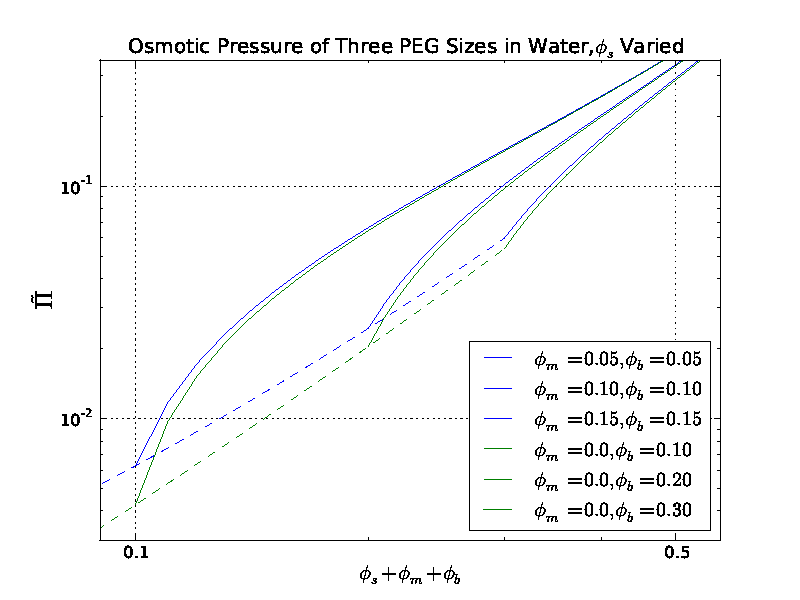
\includegraphics[width=1.0\columnwidth]{121121_OP_3_poly_loglog_phis_varied.png}}


$\Pi(\phi_s, \phi_m, \phi_b) = \frac{\overline V \Pi(\phi_s, \phi_m, \phi_b)}{k_B T} = - \mu_w = \\
= -  \ln{\left(1 - \phi_s - \phi_m, \phi_b\right)} - \phi_s - \phi_m - \phi_b + \frac{\phi_s}{N_s} + \frac{\phi_m}{N_s} + \frac{\phi_b}{N_b} \\ 
-{\textstyle\frac12}\left(\phi_s + \phi_m + \phi_b \right)^{2} + {\textstyle\frac{5}{4}} \alpha \left( {\textstyle\frac12} - \chi\right)^{3/4} \left( \phi_s + \phi_m + \phi_b\right)^{9/4}.$\\ 


D[\text{n$\_$w}*\log (\text{phi$\_$w})+\text{n$\_$s}*\log (\text{phi$\_$s})+\text{n$\_$m}*\log (\text{phi$\_$m})+\text{n$\_$b}*\log (\text{phi$\_$b})+ \text{chi}*(\text{n$\_$w} + \text{n$\_$s}*\text{N$\_$s} +\text{n$\_$m}*\text{N$\_$m} +\text{n$\_$b}*\text{N$\_$b})*(\text{phi$\_$s} + \text{phi$\_$m} + \text{phi$\_$b}) - (1/2)*(\text{n$\_$w} + \text{n$\_$s}*\text{N$\_$s} +\text{n$\_$m}*\text{N$\_$m} +\text{n$\_$b}*\text{N$\_$b})*(\text{phi$\_$s} + \text{phi$\_$m} + \text{phi$\_$b}){}^{\wedge}2 + \text{alpha}*(\text{n$\_$w} + \text{n$\_$s}*\text{N$\_$s} +\text{n$\_$m}*\text{N$\_$m} +\text{n$\_$b}*\text{N$\_$b})*((1/2)- \text{chi}){}^{\wedge}(3/4)(\text{phi$\_$s} + \text{phi$\_$m} + \text{phi$\_$b}){}^{\wedge}(9/4),\text{n$\_$w}]

\text{chi} (\text{phi$\_$b}+\text{phi$\_$m}+\text{phi$\_$s})-\frac{1}{2} (\text{phi$\_$b}+\text{phi$\_$m}+\text{phi$\_$s}){}^2+\text{alpha} \left(\frac{1}{2}-\text{chi}\right)^{3/4} (\text{phi$\_$b}+\text{phi$\_$m}+\text{phi$\_$s}){}^{9/4}+\log  \text{phi$\_$w}

D[\text{n$\_$w}*\log (\text{phi$\_$w})+\text{n$\_$s}*\log (\text{phi$\_$s})+\text{n$\_$m}*\log (\text{phi$\_$m})+\text{n$\_$b}*\log (\text{phi$\_$b})+ \text{chi}*(\text{n$\_$w} + \text{n$\_$s}*\text{N$\_$s} +\text{n$\_$m}*\text{N$\_$m} +\text{n$\_$b}*\text{N$\_$b})*(\text{phi$\_$s} + \text{phi$\_$m} + \text{phi$\_$b}) - (1/2)*(\text{n$\_$w} + \text{n$\_$s}*\text{N$\_$s} +\text{n$\_$m}*\text{N$\_$m} +\text{n$\_$b}*\text{N$\_$b})*(\text{phi$\_$s} + \text{phi$\_$m} + \text{phi$\_$b}){}^{\wedge}2 + \text{alpha}*(\text{n$\_$w} + \text{n$\_$s}*\text{N$\_$s} +\text{n$\_$m}*\text{N$\_$m} +\text{n$\_$b}*\text{N$\_$b})*((1/2)- \text{chi}){}^{\wedge}(3/4)(\text{phi$\_$s} + \text{phi$\_$m} + \text{phi$\_$b}){}^{\wedge}(9/4),\text{n$\_$s}]

\log  \text{phi$\_$s}+\text{chi} \text{N$\_$s} (\text{phi$\_$b}+\text{phi$\_$m}+\text{phi$\_$s})-\frac{1}{2} \text{N$\_$s} (\text{phi$\_$b}+\text{phi$\_$m}+\text{phi$\_$s}){}^2+\text{alpha} \left(\frac{1}{2}-\text{chi}\right)^{3/4} \text{N$\_$s} (\text{phi$\_$b}+\text{phi$\_$m}+\text{phi$\_$s}){}^{9/4}

D[\text{n$\_$w}*\log (\text{phi$\_$w})+\text{n$\_$s}*\log (\text{phi$\_$s})+\text{n$\_$m}*\log (\text{phi$\_$m})+\text{n$\_$b}*\log (\text{phi$\_$b})+ \text{chi}*(\text{n$\_$w} + \text{n$\_$s}*\text{N$\_$s} +\text{n$\_$m}*\text{N$\_$m} +\text{n$\_$b}*\text{N$\_$b})*(\text{phi$\_$s} + \text{phi$\_$m} + \text{phi$\_$b}) - (1/2)*(\text{n$\_$w} + \text{n$\_$s}*\text{N$\_$s} +\text{n$\_$m}*\text{N$\_$m} +\text{n$\_$b}*\text{N$\_$b})*(\text{phi$\_$s} + \text{phi$\_$m} + \text{phi$\_$b}){}^{\wedge}2 + \text{alpha}*(\text{n$\_$w} + \text{n$\_$s}*\text{N$\_$s} +\text{n$\_$m}*\text{N$\_$m} +\text{n$\_$b}*\text{N$\_$b})*((1/2)- \text{chi}){}^{\wedge}(3/4)(\text{phi$\_$s} + \text{phi$\_$m} + \text{phi$\_$b}){}^{\wedge}(9/4),\text{n$\_$m}]

\log  \text{phi$\_$m}+\text{chi} \text{N$\_$m} (\text{phi$\_$b}+\text{phi$\_$m}+\text{phi$\_$s})-\frac{1}{2} \text{N$\_$m} (\text{phi$\_$b}+\text{phi$\_$m}+\text{phi$\_$s}){}^2+\text{alpha} \left(\frac{1}{2}-\text{chi}\right)^{3/4} \text{N$\_$m} (\text{phi$\_$b}+\text{phi$\_$m}+\text{phi$\_$s}){}^{9/4}

D[\text{n$\_$w}*\log (\text{phi$\_$w})+\text{n$\_$s}*\log (\text{phi$\_$s})+\text{n$\_$m}*\log (\text{phi$\_$m})+\text{n$\_$b}*\log (\text{phi$\_$b})+ \text{chi}*(\text{n$\_$w} + \text{n$\_$s}*\text{N$\_$s} +\text{n$\_$m}*\text{N$\_$m} +\text{n$\_$b}*\text{N$\_$b})*(\text{phi$\_$s} + \text{phi$\_$m} + \text{phi$\_$b}) - (1/2)*(\text{n$\_$w} + \text{n$\_$s}*\text{N$\_$s} +\text{n$\_$m}*\text{N$\_$m} +\text{n$\_$b}*\text{N$\_$b})*(\text{phi$\_$s} + \text{phi$\_$m} + \text{phi$\_$b}){}^{\wedge}2 + \text{alpha}*(\text{n$\_$w} + \text{n$\_$s}*\text{N$\_$s} +\text{n$\_$m}*\text{N$\_$m} +\text{n$\_$b}*\text{N$\_$b})*((1/2)- \text{chi}){}^{\wedge}(3/4)(\text{phi$\_$s} + \text{phi$\_$m} + \text{phi$\_$b}){}^{\wedge}(9/4),\text{n$\_$b}]

\log  \text{phi$\_$b}+\text{chi} \text{N$\_$b} (\text{phi$\_$b}+\text{phi$\_$m}+\text{phi$\_$s})-\frac{1}{2} \text{N$\_$b} (\text{phi$\_$b}+\text{phi$\_$m}+\text{phi$\_$s}){}^2+\text{alpha} \left(\frac{1}{2}-\text{chi}\right)^{3/4} \text{N$\_$b} (\text{phi$\_$b}+\text{phi$\_$m}+\text{phi$\_$s}){}^{9/4}
%
%\begin{eqnarray}
%\frac{\overline V \Pi(\phi_s, \phi_m, \phi_b)}{k_B T} &=& - \mu_w = \\
%&=& -  \ln{\left(1 - \phi_s - \phi_m, \phi_b\right)} - \phi_s - \phi_m - \phi_b + \frac{\phi_s}{N_s} + \frac{\phi_m}{N_s} + \frac{\phi_b}{N_b} \\ 
%-{\textstyle\frac12}\left(\phi_s + \phi_m + \phi_b \right)^{2} + {\textstyle\frac{5}{4}} \alpha \left( {\textstyle\frac12} - \chi\right)^{3/4} \left( \phi_s + \phi_m + \phi_b\right)^{9/4}. \nonumber\\
%~
%\end{eqnarray}


        \item[\bf{Fig 2.}] Osmotic Pressure- fixed Volume Fractions for PEG100, PEG10k, increasing PEG1k:\\
		\centerline{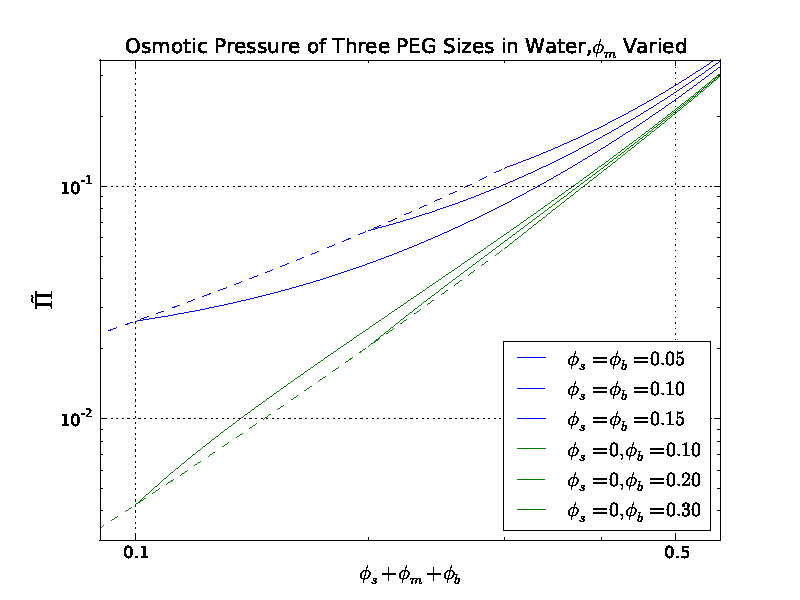
\includegraphics[width=1.0\columnwidth]{121121_OP_3_poly_loglog_phim_varied.png}}
		
		%

        \item[\bf{Fig 3.}] Partition Coefficients for PEG100 (no PEG1k in pore) and PEG1k (no PEG100 in pore), increasing PEG100 in bath:\\
		\centerline{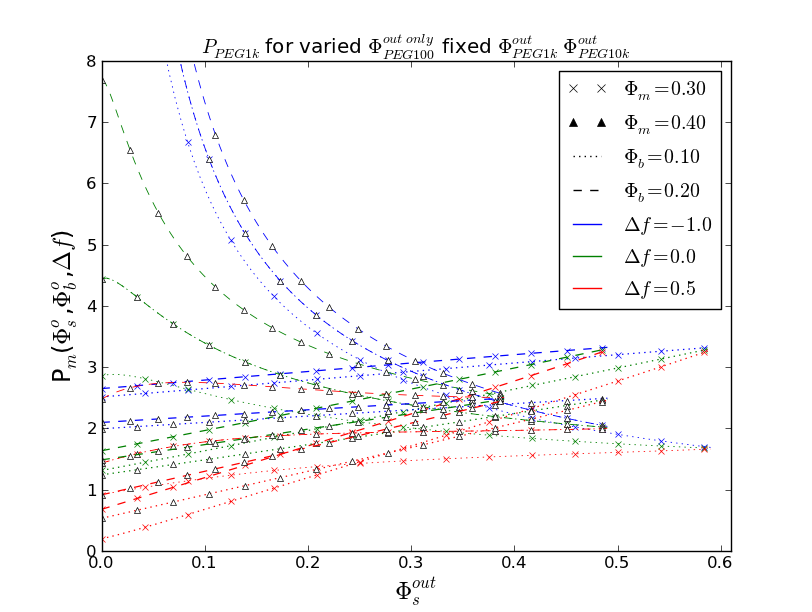
\includegraphics[width=1.0\columnwidth]{Ps_Pm_varied_phis_out_only.png}}

\begin{equation}
\mu_s (I) + \Delta f = \mu_s(O).
\label{grapel1}
\end{equation}
Also, since the solvent is in chemical equilibrium too, we need to have an additional equation
\begin{equation}
\mu_w (I) = \mu_w(O).
\end{equation}
In principle at least, here too we could add a pore penetration energy. For now we do not explore this venue. The above two equations can then be rewritten in an equivalent form
\begin{equation}
\mu_{s}(I) - N_s \mu_w(I) + \Delta f = \mu_{s}(O) - N_s \mu_w(O) 
\end{equation}
Taking into account the previous results Eq. \ref{mu1} we end up with the following equation for the pore equilibrium
\begin{eqnarray}
& & \ln{\phi_{s}(I)} - N_s (\ln{\phi_w(I)} +1 - \phi_w(I)) + N_s \frac{9}{4} \tilde\alpha \left( \phi_s(I) + \phi_b(I)\right)^{5/4} + \Delta f = \nonumber\\
&& \ln{\phi_{s}(O)} - N_s (\ln{\phi_w(O)} +1 - \phi_w(O)) + N_s \frac{9}{4} \tilde\alpha \left( \phi_s(O) + \phi_b(O)\right)^{5/4}
\end{eqnarray}
where we took out all the irrelevant constants. Also since by assumption the big polymer can not penetrate the pore $ \phi_b(I) = 0$. Therefore
\begin{eqnarray}
& & \ln{\phi_{s}(I)} - N_s (\ln{(1-\phi_{s}(I))} +\phi_{s}(I)) + N_s \frac{9}{4} \tilde\alpha \phi_s(I)^{5/4} + \Delta f = \nonumber\\
&& \ln{\phi_{s}(O)} - N_s (\ln{(1 - \phi_s(O) - \phi_b(O))} + \phi_s(O) + \phi_b(O)) + N_s \frac{9}{4} \tilde\alpha \left( \phi_s(O) + \phi_b(O)\right)^{5/4}\nonumber\\
~
\end{eqnarray}
This we can rewritten in the following way
\begin{eqnarray}
& & \ln\frac{\phi_{s}(I)}{\phi_{s}(O)} + \Delta f  = \nonumber\\
& & N_s \left( \ln\frac{(1 - \phi_s(I))}{(1 - \phi_s(O) - \phi_b(O))} + (\phi_{s}(I) - \phi_s(O) - \phi_b(O))+ \frac{9}{4} \tilde\alpha \left( \left( \phi_s(O) + \phi_b(O)\right)^{5/4} - \phi_s(I)^{5/4}\right)\right). \nonumber\\
~
\end{eqnarray}
In terms of the partition coefficient that is defined as
$$p = {\frac{\phi_s(I)}{\phi_s(O)}},$$we finally remain with
\begin{eqnarray}
\ln{p} + \Delta f &=& N_s \left( \ln\frac{(1 - p\phi_s(O))}{(1 - \phi_s(O) - \phi_b(O))} + (p\phi_{s}(O) - \phi_s(O) - \phi_b(O))+ \right.\nonumber\\
&& \left. + \frac{9}{4} \tilde\alpha \left( \left( \phi_s(O) + \phi_b(O)\right)^{5/4} - (p\phi_s(O))^{5/4} \right)\right).
\label{defp1}
\end{eqnarray}

                %$Length_{1}$ at 0$^{\circ}$ = 1,000 ft \\

        \item[\bf{Fig 4.}] Partition Coefficient for PEG100 (no PEG1k in pore), increasing PEG100 in bath:\\
		\centerline{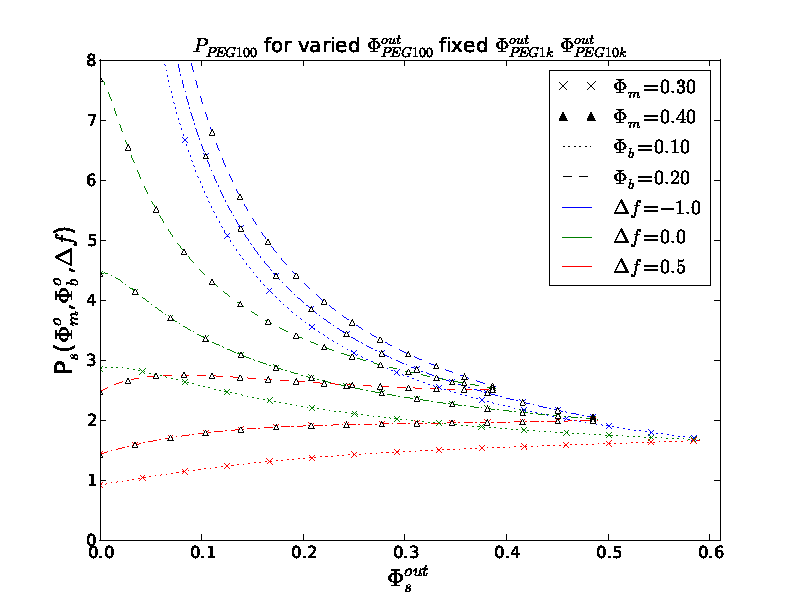
\includegraphics[width=1.0\columnwidth]{121128_PC_3_poly_Ps_in_vs_phis_out_only.png}}


                $Length_{1}$ at 0$^{\circ}$ = 1,000 ft \\

        \item[\bf{Fig 5.}] Partition Coefficient for PEG1k (no PEG100 in pore), increasing PEG100 in bath:\\
		\centerline{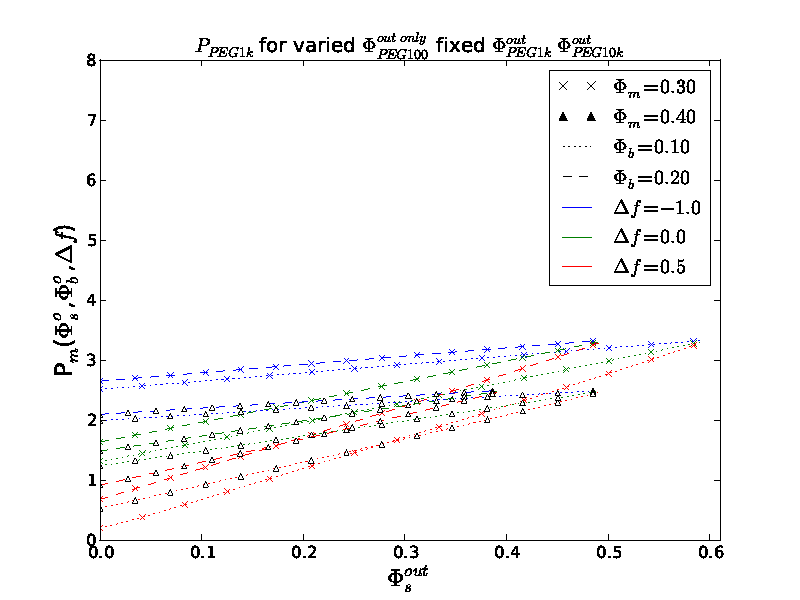
\includegraphics[width=1.0\columnwidth]{121128_PC_3_poly_Pm_in_vs_phis_out_only.png}}


                $Length_{1}$ at 0$^{\circ}$ = 1,000 ft \\

        \item[\bf{Fig 6.}] Volume Fraction of PEG1k in pore (no PEG100 in pore), increasing PEG100 in bath:\\
		\centerline{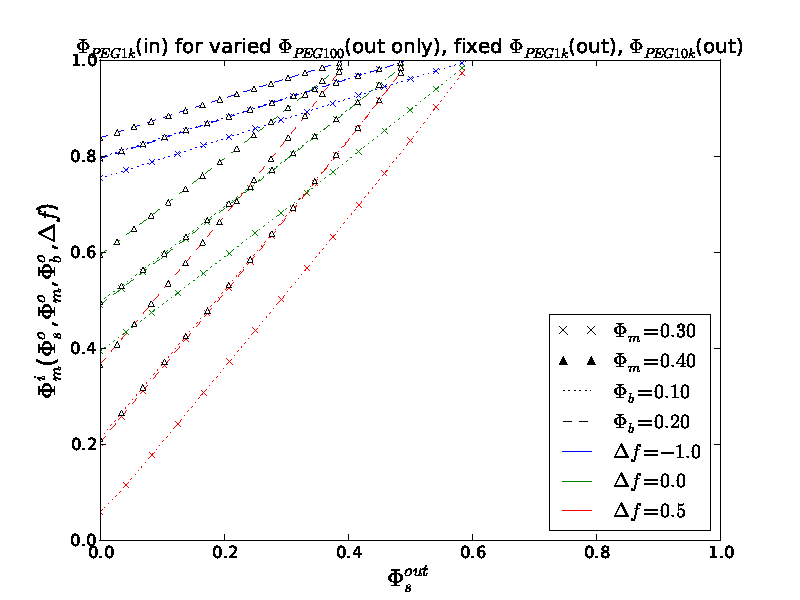
\includegraphics[width=1.0\columnwidth]{121128_PC_3_poly_phim_in_vs_phis_out_only.png}}


                $Length_{1}$ at 0$^{\circ}$ = 1,000 ft \\

        \item[\bf{Fig 7.}] Partition Coefficient for PEG1k in Pore, increasing PEG100 in bath and pore:\\
		\centerline{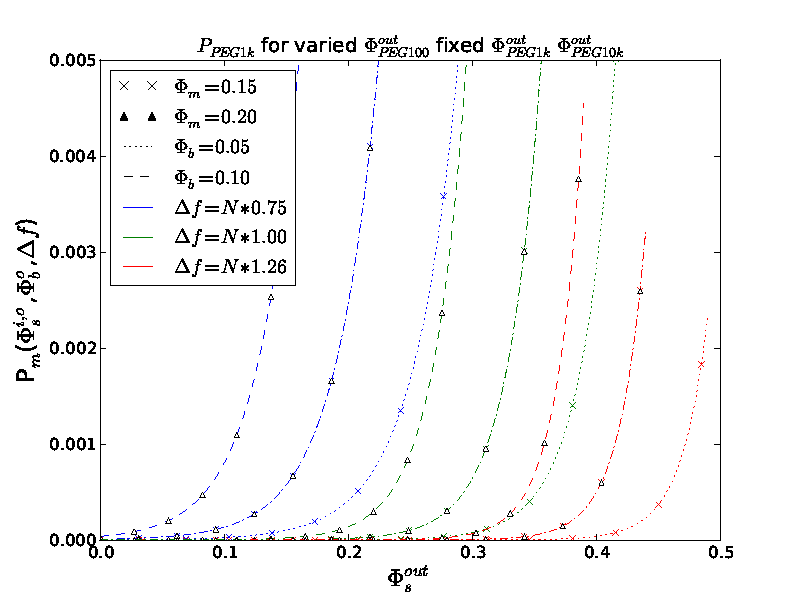
\includegraphics[width=1.0\columnwidth]{121129_PC_3_poly_Pm_in_with_true_phis_at_2300hr.png}}

%
%                $Length_{1}$ at 0$^{\circ}$ = 1,000 ft \\
%		Use:\\
%		$L_{1}$ = original length\\
%		$T_{1}$ = original temperature\\
%                $L_{2}$ = new length\\
%		$T_{2}$ = new temperature\\
%		%
%
%		$L_{2}-L_{1} = \Delta$L = change in length \\
%		$T_{2}-T_{1} = \Delta$T = change in temperature \\
%		%
%
%		$\Delta L = L_{2}-L_{1} = \alpha \times L_{1} \times (T_{2}-T{1}) = \alpha L_{1} \Delta T = \\
%		\frac{12\times10^{-6}}{degree} \times 1000 ft \times (33^{\circ}-0^{\circ}) = 0.396 ft$\\
%	%
%
%	\item [A1.] $c$ '0.4 feet'\\ \\
%%
%
%        \item[\bf{Q2.}] We are given:\\
%                %
%                $L_{1} at T_{1}=20^{\circ}$ = 30 m \\
%		Coefficient of linear expansion = $\alpha$ = 25 $\times 10^{-6}$/degree \\
%		%
%
%		We want to find $T_{2}$ when $L_{2}$ = (30 m - 0.05 m) = 29.95 m \\
%		%
%
%		Use the same equation we used in Q1 but with $\alpha$ = 25 $\times 10^{-6}$/degree:\\
%		%
%		$\Delta L = \alpha L_{1} \Delta T = \frac{25\times10^{-6}}{degree} \times 30 m \times \Delta T$, where $\Delta L$ = -0.05 m\\ 
%		(negative because the wing got shorter when it got colder)\\
%		%
%		
%		Solve for $\Delta T$: \\
%		$\Delta T = (-0.05 m)\times \frac{degree}{25 \times 10^{-6}} \times \frac{1}{30 m} = -66.67^{\circ}$ \\
%		%
%		
%		We know:\\ 
%		$\Delta T = T_{2}-T_{1}$ and that $T_{1} = 20^{\circ}$ \\
%		%
%
%		Solve for $T_{2}$ using: \\		
%		%
%		$-66.67^{\circ} = T_{2}-20^{\circ}$\\
%		so,  $T_{2} = -46.67^{\circ}$\\
%		%
%
%	\item [A2.] $d$ '$-45^{\circ}$'\\ \\
%%
%
%        \item[\bf{Q3.}] We are given:\\
%		%
%		$\Delta W$ = -100 J\\ 
%		(Note: We are given the amount of work done $\underline{BY}$ the balloon, but for our calculations, we want to use the amount of work $\underline{ON}$ the balloon, this is the reason for the negative sign here.)\\
%		$\Delta Q$ = 140 J\\
%		$\Delta U$ = ?\\
%		%
%		
%		Use:\\
%		$\Delta U \equiv \Delta W + \Delta Q = -100J + 140J = +40 J$\\
%		%
%
%	\item[A3.] $c$ '+40 J'\\ \\
%%
%
%        \item[\bf{Q4.}] We're given:\\
%		m = 2 kg\\
%		$T_{1} = 20^{\circ}$\\
%		$T_{2} = 220^{\circ}$\\
%		c = 390 $\frac{J}{kg \cdot K^{\circ}}$\\
%		%
%
%		Use:\\ 
%		$Q = c \times m \times (T_{2}-T_{1}) = (390 \frac{J}{kg \cdot K^{\circ}})(2 kg)(200^{\circ}) =$\\ 
%		$390 J \times 2 \times 200 = 156,000 J = 156 kJ$ \\ 
%		%
%	\item[A4.] $c$ '150 kJ'\\ \\
%%
%
%        \item[\bf{Q5.}] We're given:\\
%		m = 3 kg\\
%		$T_{1} = 20^{\circ}$\\
%		$T_{2} = 3^{\circ}$\\
%		c = 4,180 $\frac{J}{kg \cdot K^{\circ}}$\\
%		$\Delta Q$ = ?\\
%		%
%
%		Use same equation as Q4:\\ 
%		$\Delta Q = c \times m \times \Delta T = (4180 \frac{J}{kg \cdot K^{\circ}})(3 kg)(3^{\circ} - 20^{\circ}) = $\\
%		$4180 J \times 3 \times -17 = -213,180 J = -213 kJ \approx -200 kJ$ \\
%		%
%
%		Note: We don't need to keep the negative sign in the answer because the question asks how mush is "removed", so the negative sign is implied in the answer\\
%		%
%	\item[A5.] $d$ '200 kJ'\\ \\
%%
%
%        \item[\bf{Q6.}] We're given:\\
%		m = 1 kg\\
%		$T_{1} = 20^{\circ}$\\
%		$T_{2} = 660^{\circ}$\\
%		c = 890 $\frac{J}{kg \cdot K^{\circ}}$\\
%		$\Delta Q$ = ?\\
%		%
%
%		Use same equation again:\\ 
%		$\Delta Q = c \times m \times \Delta T = (890 \frac{J}{kg \cdot K^{\circ}})(1 kg)(660^{\circ} - 20^{\circ}) = 890 J \times 640 = 569,600 J = 570 kJ \approx 580 kJ$ \\
%		%
%
%	\item[A6.] $d$ '580 kJ'\\ \\
%%
%
%       \item[\bf{Q7.}] We're given: \\
%		%
%		m = 10 kg\\
%		$\Delta h$ = (10 m - 0 m) = 10 m\\
%		%
%
%		To turn mass in to a force, use:\\
%		$F = ma = (10 kg)(9.8 m/s^{2}) = 98 N$\\
%		%
%		
%		To find the work done, use:\\
%		$Work = Force \times distance = 98 N \times 10 m = 980 J \approx 1000 J = 1 kJ$\\
%		% 
%	\item[A7.] $c$ '1 kiloJoule'\\ \\
%%
%
%        \item[\bf{Q8.}] We're given:\\
%		m = 10 kg\\
%		$T_{1} = 20^{\circ}$\\
%		$T_{2} = 30^{\circ}$\\
%		c = 4180 $\frac{J}{kg \cdot K^{\circ}}$\\
%		$\Delta Q$ = ?\\
%		%
%
%		Use same equation as Q4:\\ 
%		$\Delta Q = c \times m \times \Delta T = (4180 \frac{J}{kg \cdot K^{\circ}})(10 kg)(10^{\circ}) = 418 kJ \approx 400 kJ$ \\
%		%
%	\item[A8.] $d$ '400 kJ'\\ \\
%%
%
%        \item[\bf{Q9.}] We are given:\\		
%		%
%		$\Delta W$ = 1 kJ\\
%		$\Delta Q$ = 400 kJ\\	
%		%
%
%		$H_{F}$ = latent heat of fusion = it takes 334 kJ to melt 1 kg of ice\\
%		%
%
%		Find the $\Delta Q$ need to freeze 10 kg of water: \\
%		To calculate the amount of heat to freeze (or melt) water (or ice) use the following equation,\\
%		$\Delta Q = m \times H_{F} = 10kg \times \frac{334 kJ}{1 kg} = 3340 kJ$\\
%		%
%
%	\item[A9.] $c$ '3340 kJ'\\ \\ 
%%
%
%        \item[\bf{Q10.}] We are given:\\		
%		%
%		$H_{V}$ = latent heat of vaporization = 2260 kJ/kg\\
%		$\Delta Q = m \times H_{V} = 10 kg \times 2260 \frac{kJ}{kg} = 22600 kJ$\\	
%		%
%
%		Note: there was a typo in the original version of this homework set. The question was corrected to read "How many times more heat does it take to boil vs to melt a given amount of water?"\\
%		%
%
%		The latent heat of vaporization is how much heat you would need to add to a given mass of water to make it undergo a phase change from liquid to vapor.  In other words, to boil water on a stove, you put the cold water on the burner, the burner adds heat, causing the water to warm up. When the water gets close to its boiling temperature, the burner must add more heat than it had been in order to increase the temperature of the water so that it boils and makes vapor(steam).\\
%		%
%
%		The analog is true for the latent heat of fusion; it's the amount of heat you would need to make ice undergo a phase change into water.\\
%		%
%
%		We just calculated $\Delta Q_{to\:boil} = 22600 kJ$ for 10 kg of water\\
%		In Q9, we found $\Delta Q_{to\:melt} = 3340 kJ$ for 10 kg of ice\\
%		%
%
%		To find how many times more heat you'll need to boil some mass of water vs how much heat you'll need to melt some ice with the same mass:\\
%		\centerline{$\frac{\Delta Q_{to \: boil}}{\Delta Q_{to \: melt}} = \frac{22600 kJ}{3340 kJ} = 6.67 \approx 7 times $}\\
%		%
%
%		Knowing that water boils at 100$^\circ$C, it takes a lot more heat to make it boil (i.e. to bring it through the boiling point, for example, to heat it from 99$^\circ$C to 101$^\circ$C) than to make it just bit hotter (i.e. to go from 96$^\circ$C to 98$^\circ$ degrees C).  The analog is true for melting, you have to put in a lot of heat to make ice go from just barely frozen to just barely melted. This problem shows us that the amount of heat to cause water to boil is a lot more than the amount of heat to make ice melt.\\
%		%
%	\item[A10.] $b$ 'it takes 7 times as much heat to boil vs melt water'\\ \\ 
%%
%
%        \item[\bf{Q11.}] Use the Ideal Gas Equation:\\		
%		%
%
%		\centerline{$Pressure \times Volume = (constant) \times Temperature$},\\
%		%
% 
%		where $constant = Nk$ (number of particles,N; Boltzmann constant,k)\\
%		%
%
%		Rearrange the equation so that the constant is the only thing on the right hand side:\\
%		%
%
%		$\frac{PV}{T} = constant$\\ 
%		%
%		This means that for an ideal gas, if you change the pressure, volume and/or temperature, the other variables must accomodate that change so that $\frac{PV}{T}$ always equals the same number.\\
%		%
%
%		Let $P_{1}, V_{1}$ be the pressure and volume that you measured before compressing the gas\\
%		%
%
%		Let $P_{2}, V_{2}$ be the pressure and volume after compressing it to half of $V_{1}$, where $V_{2}=\frac{1}{2}V_{1}$\\
%		%
%
%		Use:\\
%		%
%		\centerline{$\frac{P_{1} V_{1}}{T} =constant= \frac{P_{2} V_{2}}{T}$},\\ 
%		where $V_{2} = \frac{1}{2}V_{1}$ and T is the same before and after compression.\\ 
%		%
%	
%		Plug in $\frac{1}{2}V_{1}$ for $V_{2}$ in the right hand side of the equation:\\
%		\centerline{$\frac{P_{1} V_{1}}{T} =constant= \frac{P_{2} \frac{1}{2}V_{1}}{T}$}\\
%		%
%
%		Cancel out the like terms on both sides of the eqn and solve for $P_{2}$:\\
%		\centerline{$P_{2} = 2 \times P_{1}$}\\
%		%
%
%		$P_{2}$ is twice as much pressure as $P_{1}$, this means that you must increase $P_{1}$ by adding 100 percent more of it.\\
%		%
%
%		Note: $P_{2}$ is 200 percent of $P_{1}$ but the question asks how much you need to $\underline{increase}$ the pressure. You need to add  100 percent more of $P_{1}$ to get $P_{2}$.\\
%		%
%	\item[A11.] $c$ '100 percent'\\ \\ 
%%
%
%        \item[\bf{Q12.}] We're given the temperatures in Celsius, convert to Kelvin by adding $273^{\circ} \approx 300^{\circ}$:\\
%		%
%
%		$T_{1} = T_{hot} = 100^{\circ}C \approx 400^{\circ}$ Kelvin\\
%		$T_{2} = T_{cold} = 0^{\circ}C \approx 100^{\circ}$ Kelvin\\
%		%
%
%		Note: there was a typo in the original version, the efficiency cannot be more than 1.\\
%		%
%
%		Use:\\
%		Efficiency  = $\eta = \frac{Work \: done}{Heat \: added}$\\
%		Carnot Efficiency = $\eta_{carnot} = \frac{T_{hot}-T_{cold}}{T_{hot}} = \frac{400^{\circ}-300^{\circ}}{400^{\circ}} = \frac{1}{4} = 25$ percent\\
%		%
%	\item[A12.] $a$ '25 percent'\\ \\
%%

\end{itemize}
\end{document}

